\documentclass[12pt]{article}
\usepackage[]{cite}
\usepackage{cmap}
\usepackage[T2A]{fontenc}
\usepackage[utf8]{inputenc}
\usepackage[english, russian]{babel}
\usepackage{amsmath, amsfonts,amssymb}
\usepackage{graphicx, epsfig}
% \usepackage{subfig}
\usepackage{subcaption}
\usepackage{color}
\usepackage{hyperref}


% \newcommand\argmin{\mathop{\arg\min}}
% \newcommand{\T}{^{\text{\tiny\sffamily\upshape\mdseries T}}}
% \newcommand{\hchi}{\hat{\boldsymbol{\chi}}}
% \newcommand{\hphi}{\hat{\boldsymbol{\varphi}}}
% \newcommand{\bchi}{\boldsymbol{\chi}}
% \newcommand{\A}{\mathbf{A}}
% \newcommand{\bb}{\mathbf{b}}
% \newcommand{\B}{\mathcal{B}}
% \newcommand{\W}{\mathbf{W}}
% \newcommand{\E}{\mathbf{E}}
\newcommand{\x}{\mathbf{x}}
\newcommand{\y}{\mathbf{y}}
\newcommand{\Y}{\mathbf{Y}}
\newcommand{\X}{\mathbf{X}}
\newcommand{\D}{\mathcal{D}}
\newcommand{\s}{\mathbf{s}}
% \newcommand{\Z}{\mathbf{Z}}
% \newcommand{\hx}{\hat{x}}
% \newcommand{\hX}{\hat{\X}}
% \newcommand{\hy}{\hat{y}}
\newcommand{\M}{\mathcal{M}}
\newcommand{\I}{\mathcal{I}}
\newcommand{\Q}{\mathcal{Q}}
\renewcommand{\S}{\mathcal{S}}
% \newcommand{\N}{\mathcal{N}}
\newcommand{\R}{\mathbb{R}}
% \newcommand{\p}{p(\cdot)}
% \newcommand{\cc}{\mathbf{c}}
% \newcommand{\m}{\mathbf{m}}
% \newcommand{\bt}{\mathbf{t}}
% \newcommand{\e}{\mathbf{e}}
% \newcommand{\h}{\mathbf{h}}
% \newcommand{\q}{q(\cdot)}
% \newcommand{\uu}{\mathbf{u}}
% \newcommand{\vv}{\mathbf{v}}
% \newcommand{\dd}{\partial}

\renewcommand{\baselinestretch}{1}


\newtheorem{Th}{Теорема}
\newtheorem{Def}{Определение}
\newenvironment{Proof} % имя окружения
    {\par\noindent{\bf Доказательство.}} % команды для \begin
    {\hfill$\scriptstyle\blacksquare$} % команды для \end
\newtheorem{Assumption}{Предположение}
\newtheorem{Corollary}{Следствие}

\textheight=24cm % высота текста
\textwidth=16cm % ширина текста
\oddsidemargin=0pt % отступ от левого края
\topmargin=-1.5cm % отступ от верхнего края
\parindent=24pt % абзацный отступ
\parskip=0pt % интервал между абзацами
\tolerance=2000 % терпимость к "жидким" строкам
\flushbottom % выравнивание высоты страниц

%\graphicspath{ {fig/} }



\begin{document}

\thispagestyle{empty}
\begin{center}
    \sc
        Министерство образования и науки Российской Федерации\\
        Московский физико-технический институт
        {\rm(государственный университет)}\\
        Физтех-школа прикладной математики и информатики\\
        Кафедра <<Интеллектуальные системы>>\\
        Направление <<Интеллектуальный анализ данных>> \\[30mm]
    \rm\large
        Соболевский Федор Александрович\\
        Б05-111\\[10mm]
    \bf\Large
	Применение больших языковых моделей 
        для иерархической суммаризации
        текстов научных публикаций \\[10mm]
    \rm\normalsize
    \sc
        Выпускная квалификационная работа бакалавра\\[10mm]
\end{center}
\hfill\parbox{90mm}{
    \begin{flushleft}
    \bf
        Научный руководитель:\\
    \rm
        д.~ф.-м.~н. Воронцов Константин Вячеславович\\[5cm]
    \end{flushleft}
}
\begin{center}
    Москва\\
    2025
\end{center}


\newpage
\tableofcontents
\newpage

\begin{abstract}
В век экспоненциального роста количества доступной информации в мире особенно актуальной становится задача структурирования и систематизации научных знаний, а также повышения их доступности. Иерархическая организация основных идей и результатов в научных публикациях может позволить ускорить процесс получения читателем знаний и позволить ему двигаться при изучении темы от главного к деталям. Одним из видов структурированного представления текста являются интеллект-карты на основе предложений. Поскольку человеческая обработка больших коллекций текстовых документов, особенно научных, занимает много времени и ресурсов, для решения задачи иерархической суммаризации необходимо разрабатывать автоматические методы, по качеству не уступающие ручной обработке. 

Перспективным инструментом решения данной задачи являются большие языковые модели. В данной работе исследуется способность больших языковых моделей строить иерархические представления текстов научных публикаций на примере интеллект-карт. Поскольку для задачи автоматической иерархической суммаризации научных текстов на данный момент не существует достаточного количества обучающих данных и метрик для разностороннего и полного оценивания качества генерации, предварительно проводится работа по созданию новой коллекции иерархических сводок научных статей для обучения и тестирования моделей иерархической суммаризации и предлагаются новые способы оценивания результатов выполнения данной задачи.

  \bigskip
  \textbf{Ключевые слова}: \emph{большие языковые модели, иерархическая суммаризация, интеллект-карты
  }
\end{abstract}

\newpage

%%%%%%%%%%%%%%%%%%%%%%%%%%%%%%%%%%%%%%%%%%%%%%%%%%%%%%%%%%%%%%%%%%%%%%%%%%%%%
\section*{Введение}
\addcontentsline{toc}{section}{\protect\numberline{}Введение}

\paragraph{Актуальность темы.} 
\textit{TO-DO}

\textit{- большие объемы информации, дезинформации и необходимость структурирования её}

\textit{- необходимость более эффективного распространения новых научных знаний}


\textit{- эффективность интеллект-карт из предложений как инструмента эффективного получения новых знаний и при этом практическое отсутствие выборок и информативных метрик для задачи иерархической суммаризации.}

\textit{- быстрое развитие больших языковых моделей, их SOAT результаты в сфере суммаризации и нераскрытый потенциал для задачи иерархической суммаризации.}

\paragraph{Цели работы.}
\begin{itemize}
    \item Формализовать задачу автоматического построения интеллект-карт по научным публикациям и предложить метрики оценивания таких карт, достаточно хорошо отражающие реальное качество генерации по структуре, связности и достоверности;
    \item Разработать и применить методику построения интеллект-карт по научным текстам экспертами с целью формирования выборки - золотого стандарта для обучения и валидации моделей автоматической иерархической суммаризации, а также с целью выработки четких требований и целей для автоматической генерации;
    \item Применить большие языковые модели (БЯМ) для генерации интеллект-карт по текстам научных статей и определить оптимальные запросы, позволяющие максимизировать качество генерации для каждой выбранной БЯМ;
    \item Проанализировать свойства генерируемых с помощью БЯМ карт, их достоинства и недостатки самих по себе и в сравнении со стандартами и определить границы применимости современных БЯМ для иерархической суммаризации научной литературы. 
\end{itemize}


\paragraph{Методы исследования.}
\textit{TO-DO}


\paragraph{Основные положения, выносимые на защиту.}
\textit{TO-DO}


\paragraph{Научная новизна.}
\textit{TO-DO}

\textit{to my best knowledge, на данный момент нет ни адекватных критериев для автоматического оценивания карт знаний по научным статьям, ни выборки для данной задачи}


\paragraph{Теоретическая значимость.}
\textit{TO-DO}

\textit{- формализация задачи гибридной иерархической суммаризации в виде интеллект-карт из предложений}

\textit{- разработка автоматических метрик оценки качества иерархических представлений текста по собственной структуре карты и в сравнении с референсом}


\paragraph{Практическая значимость.}
\textit{TO-DO}

\textit{- разработка метода автоматической генерации представлений научных статей для их эффективного изучения с нужной степенью углубления в детали}

\textit{- датасет для задачи генерации интеллект-карт из предложений по научным текстам}

\textit{- (было бы неплохо?) фреймворк для автоматического оценивания подобных интеллект-карт}


\paragraph{Степень достоверности и апробация работы.}
\textit{TO-DO}

%%%%%%%%%%%%%%%%%%%%%%%%%%%%%%%%%%%%%%%%%%%%%%%%%%%%%%%%%%%%%%%%%%%%%%%%%%%%%
\newpage
\section*{Обозначения и сокращения}
\addcontentsline{toc}{section}{\protect\numberline{}Обозначения}
\begin{itemize}
    \item \textit{БЯМ}~--- большая языковая модель (large language model);
    
    \item Под \textit{картами знаний} или \textit{интеллект-картами} в данной работе будут подразумеваться интеллект-карты на основе предложений (salient-sentence-based mind maps, SSM \cite{wei2019revealing}).

    \item \textit{KSM}~--- интеллект-карта на основе главных выдержек (key-snippet based mind map).

    \item \textit{ROUGE} - Recall-Oriented Understudy for Gisting Evaluation (статистическая метрика качества суммаризации).

    \item \textit{BLEU} - Bilingual Evaluation Understudy (статистическая метрика качества генерации текста, основное применение~--- оценка машинного перевода).

    \item \textit{ИАТ}~--- интеллектуальный анализ текста (text mining).
\end{itemize}

%%%%%%%%%%%%%%%%%%%%%%%%%%%%%%%%%%%%%%%%%%%%%%%%%%%%%%%%%%%%%%%%%%%%%%%%%%%%%
\newpage
\section{Постановка задачи}
\subsection{Задача иерархической суммаризации}
Пусть дан документ (или коллекция документов) $\D$~--- упорядоченный набор предложений, составленных из слов некоторого словаря $V$: 
$$
\D = \left(s_i\right)_{i=1}^{|\D|},\quad \text{где } \forall i=1,\dots |\D|\quad s_i = \left(w_{ij}\right)_{j=1}^{l_i}, \quad w_{ij}\in V,
$$
а также референсная карта $\M^* = (\S^*, E^*)$ и метрика качества $\I: (\M, \D, \M^*) \rightarrow \R$. Тогда требуется найти отображение $f^*: \D \rightarrow \M = (\S, E)$, максимизирующее данную метрику качества $\I$, где $\M$~--- древовидная \textbf{иерархическая карта} (\textit{интеллект-карта}, \textit{карта знаний}), $\S$~--- набор предложений, являющихся вершинами $\M$ и составленных из слов словаря $V$, $E\in \S^2$~--- направленные иерархические связи между предложениями из $\S$, то есть ребра направленного графа $\M$:
$$
f^* = \arg\max\limits_{f} \I(f(\D), \D, \M^*).
$$

\subsection{Задача разработки критериев оценки карт знаний}
Поскольку на данный момент нет четких критериев для автоматической оценки качества иерархической суммаризации в виде карт знаний, перед тестированием БЯМ необходимо разработать систему таких критериев. Пусть мы имеем сгенерированную моделью по документу $\D$ карту знаний $\M$ и карту-стандарт $\M^*$ по тому же документу, созданную экспертами. 
Требуется определить критерии $$\I_k: (\M, \D, \M^*) \rightarrow \R$$ для автоматического оценивания интеллект-карт, отражающие интересующие нас аспекты качества генерации иерархического представления $\M$ относительно исходного документа $\D$ и карты-стандарта $\M^*$. 
Мера качества критерия~--- коэффициент корреляции с экспертной метрикой $\I^*_k$ оценки соответствующего аспекта качества по некоторой выборке карт $\X$. 

Выделим пять основных реальных аспектов качества карты знаний:
\begin{itemize}
    \item \textit{соответствие цели}, для которой создаётся данное представление документа;
    \item \textit{полнота} карты относительно документа, то есть содержание в ней всей необходимой пользователю информации на любом требуемом уровне абстракции и отсутствие лишнего;
    \item \textit{непротиворечивость} иерархического представления как на уровне предложений, так и между ними;
    \item \textit{связность} и \textit{неизбыточность} карты как набора осмысленных предложений и их последовательностей (подразумевается, что любой путь из корня дерева произвольной длины представляет из себя связный, неизбыточный текст);
    \item \textit{логичность} связей между вершинами в карте: степень логической связи между соединенными ребрами предложениями и корректность иерархии с логической точки зрения. 
\end{itemize}

В предыдущей постановке задачи неизбежно возникает следующая проблема: количество экспертных карт и скорость их создания сильно ограничены, поэтому после отработки сравнительных критериев следует разработать способ оценивать карты без стандартов. 

Пусть мы имеем только документ $\D$ и сгенерированную по нему моделью карту знаний $\M$. Требуется определить собственные критерии качества карты
$$\I_k: (\M, \D) \rightarrow \R,$$ 
отражающие качество генерации иерархического представления $\M$ исходного документа $\D$ самого по себе, без сравнения с другими картами. Мерой качества автоматического критерия, помимо степени скоррелированности с экспертными оценками, может послужить также результат оценивания с помощью него экспертных карт $\M^*$, принимаемых за стандарт.

\subsection{Задача оптимизации промптинга БЯМ}
Основной инструмент оптимизации работы готовой БЯМ без её дополнительного дообучения~--- подбор оптимального текстового запроса для решения задачи (\textit{промптинг}). Поскольку на данный момент нет достаточно быстрых алгоритмов поиска по всему множеству возможных запросов, а полный перебор запросов для каждой модели занимает слишком большое время, отдельной задачей в нашей работе является оптимизация промптинга БЯМ для цели генерации интеллект-карт и в целом.

Пусть дана выборка документов $\X$, языковая модель $f$, карта-стандарт $\M^*$ для заданной цели создания карты и некоторая метрика качества $\I$. Пусть также задано множество возможных запросов $\Q$, таких что вывод модели для каждого $(\D, Q)\in\X\times\Q$ соответствует требуемому формату, и содержащих формулировку цели, \textit{общую для модели и экспертов} - создателей $\M^*$. Требуется найти оптимальный запрос $Q^*\in\Q$, такой что вывод модели при входе $(\D, Q^*)$ максимизирует метрику $\I$ по выборке $\X$:
$$
Q^* = \arg\max\limits_{Q\in\Q} \frac{1}{|\X|}\sum\limits_{\D\in\X} \I(f(\D, Q), \D, ).
$$
Для эффективного поиска оптимального запроса (\textit{промптинга}) требуется также задать полное и неизбыточное множество запросов $\Q$ и эффективную \textit{стратегию поиска оптимального запроса} в $\Q$.

\subsection{Требования к мере близости текстовых деревьев.} \label{metric_requirements}
Чтобы определить адекватную метрику на множестве текстовых деревьев, мы сформулируем некоторые требования к произвольной метрике в пространстве таких объектов. Пусть $\mathcal{S}$~--- множество всевозможных фрагментов текста. Определим текстовое дерево как дерево $T = (V, E)$, где $E \subset V^2$ и для каждой вершины $v\in V$ определена текстовая метка $s(v)\in\mathcal{S}$. Обозначим множество всевозможных текстовых деревьев за $\mathcal{T}$. Зададим функцию семантической близости текстовых фрагментов: $r: \mathcal{S}^2 \rightarrow [0, +\infty)$. Для $v, v'\in V$ обозначим $r(v, v') := r(s(v), s(v'))$, а $r(v) := r(s(v), \lambda)$, где $\lambda$~--- пустая строка. Также обозначим как $f: [0,+\infty)\rightarrow[0,+\infty)$ некоторую неубывающую функцию. Требуется определить функцию сходства $\rho: \mathcal{T}^2 \rightarrow [0, +\infty)$, отвечающую следующим требованиям учета семантической и структурной близости:
\begin{enumerate}
    \item Симметричность: $\rho(T, T') = \rho(T', T)$;
    \item Равенство нулю в случае равенства аргументов: $\rho(T, T) = 0$;
    \item Если $T'$ получено из $T$ добавлением в $T$ вершины $v$, то $\rho(T, T') = f(r(v))$;
    \item Если $T'$ получено из $T$ удалением из $T$ вершины $v$, то $\rho(T, T') = f(r(v))$;
    \item Если $T'$ получено из $T$ заменой вершины $v$ на $v'$, то $\rho(T, T')= f(r(v, v'))$;
    \item $\rho$ удовлетворяет неравенству треугольника: 
    \begin{equation} \label{metric_requirement_6}
        \forall T, T', T''\in\mathcal{T}\quad \rho(T,T'')\leq\rho(T,T')+\rho(T',T'').
    \end{equation}
\end{enumerate}

%%%%%%%%%%%%%%%%%%%%%%%%%%%%%%%%%%%%%%%%%%%%%%%%%%%%%%%%%%%%%%%%%%%%%%%%%%%%%%
\newpage
\section{Обзор}
\subsection{Методы суммаризации}

\paragraph{Суммаризация текстов и БЯМ.} Задача суммаризации текста представляет из себя задачу получения краткого представления $\S$ документа (или коллекции документов) $\D$. Выделяют два основных вида суммаризации: \textit{экстрактивную} (extractive), использующую предложения исходного документа ($\S\subset\D$), и \textit{абстрактивную}, то есть генерацию новых предложений на основе исходного текста ($\S\not\subset\D$). Также отдельно упоминается так называемая \textit{гибридная суммаризация} (hybrid summarization), подразумевающая извлечение из документа важных предложений с последующим их преобразованием. 

Хотя задача суммаризации появилась в научной литературе ещё во второй половине XX века \cite{luhn1958automatic}, основной объем работ по суммаризации текстов был опубликован уже в XXI году, причем до начала бурного развития архитектур глубокого обучения основные методы построения сводок документов и их оценки были в большинстве своем экстрактивными, основанными на статистических приемах обработки текстов \cite{allahyari2017text}. Абстрактивная суммаризация начала активно развиваться с момента появления трансформерных архитектур и других архитектур глубокой машинной обработки текста \cite{el2021automatic}. 

Особенных успехов в области удалось добиться с появлением больших языковых моделей, которые стали основным инструментом ля суммаризации текстов, так как показали значения метрик качества, которых до этого момента не удавалось добиться \cite{jin2024comprehensive}. Более того, способности БЯМ к пониманию, обработке и генерации текста нашли свое применение не только для автоматической генерации сводок, но и для их же оценивания и корректировки \cite{wu2023large}. Сравнение результатов работы БЯМ и человека по классической (линейной) суммаризации текстов на данный момент позволяет утверждать, что для некоторых типов текста машинная суммаризация с помощью БЯМ уже достигла уровня человека \cite{pu2023summarization}. Авторы данной работы, однако, подчеркивают, что проблема оценки качества нейросетевой суммаризации и генерации текста в целом до сих пор остается открытой, поэтому нельзя утверждать о полной достаточности БЯМ для суммаризации. Применимость БЯМ для других видов суммаризации текстов все еще остается мало исследованной.

\paragraph{Иерархическая суммаризация.} Идея структурированной суммаризации текстов как более эффективного способа суммаризации больших документов появилась в научной литературе еще в конце 2000-х гг. \cite{yang2008hierarchical}, однако впервые она была формализована в работе \cite{christensen2014hierarchical}. В первоначальной постановке задача иерархической суммаризации текста представляет из себя задачу генерации \textit{иерархии из сводок} по исходной коллекции документов, в которой дочерние сводки раскрывают содержание элементов (например, предложений) более общих сводок. Метод, представленный в \cite{christensen2014hierarchical}, подразумевает иерархическую кластеризацию предложений текста с последующей суммаризацией каждого кластера. Целевая функция в \cite{christensen2014hierarchical} отражает значимость выделенных предложений, неизбыточность и связность (как внутри элементов иерархии, так и между ними) полученной иерархической сводки. Хотя авторам удалось показать, что данный подход к суммаризации новостных текстов более предпочтителен среди пользователей, чем классические подходы к суммаризации новостных текстов, данная методика не получила дальнейшего развития. Более применимыми стали подходы, основанные на генерации \textit{интеллект-карт} на основе текстов.

\paragraph{Интеллект-карты.} На сегодняшний день существует множество различных видов организации знаний в виде графовых структур: онтологии, карты концепций (concept maps) и другие, но в данной работе нас будут интересовать \textit{интеллект-карты}, или \textit{карты знаний}, поскольку они являются наиболее наглядными и удобными для освоения новой информации от главного к деталям. В работах по автоматической генерации интеллект-карт выделяют два основных вида интеллект-карт: \textit{интеллект-карты на основе значимых предложений} (salient sentence-based mind maps, SSM) и \textit{интеллект-карты на основе главных выдержек} (key snippet-based mind maps, KSM). В данной работе нас будут интересовать именно SSM как форма иерархической организации \textit{фактов} (в роли которых будут выступать связные предложения), однако следует подчеркнуть, что практическая значимость интеллект-карт в образовании и других областях исследовалась больше на примере KSM. Также обратим внимание на то, что интеллект-карты при применении их человеком зачастую не ограничиваются лишь иерархиями из текста и могут содержать как более сложные структурные элементы, так и нетекстовые элементы (например, визуальные).

С момента появления в медиа термина <<mind map>> интеллект-карты были экстенсивно изучены как инструмент представления, обработки и систематизации знаний. Многочисленные исследования применения интеллект-карт в школьном и высшем образовании как для презентации информации ученикам/студентам, так и для систематизации полученных знаний им же показали, что такой способ представления информации может заметно улучшить качество восприятия, запоминания и систематизации знаний студентами, в том числе при изучении научной литературы \cite{guerrero2015mind}. Подробный современный обзор применения интеллект-карт в образовании в XXI веке можно найти, например, в \cite{mitra2023tradition}.

\textit{TO-DO: Найти ещё исследований в "многочисленные исследования"}

\paragraph{Автоматическая генерация интеллект-карт.} В последнее десятилетие появился ряд работ по автоматической суммаризации текстов в виде интеллект-карт разных видов при помощи методов машинного обучения. Стоит отметить, что до этого были работы по генерации карт знаний/онтологий по текстам методами ИАТ, но в этих работах фокус больше направлен на моделирование взаимосвязей между отдельными словами/понятиями в тексте, чем между предложениями/фактами, поэтому для нашего исследования данные работы неактуальны.

В работе \cite{wei2019revealing} был предложен метод интеллект-карт (как KSM, так и SSM) по текстам следующим способом: а) с помощью сравнения эмбеддингов предложений строится граф взаимосвязей между ними; б) по графу взаимосвязей строится интеллект-карта нужного вида. Данная идея нашла свое развитие в работе \cite{hu2021efficient}, в которой авторы предложили более эффективный способ превращения графа отношений между предложениями в интеллект-карту с помощью модуля дистилляции графа (graph refinement module). В работе \cite{zhang2024coreference} эта идея была усовершенствована применением вместо графа отношений между предложениями, строящегося по эмбеддингам предложений, графа соотнесенности (coreference graph, discourse graph), строящегося по принципу, описанному в работе \cite{xu2019discourse}. В результате в \cite{zhang2024coreference} были полученные самые высокие значения используемых метрик качества, поэтому мы можем использовать данную модель в качестве базовой для сравнения результатов, полученных с помощью БЯМ, и результатов, достижимых с помощью специализированных нейросетевых архитектур.

В недавнее время были начаты исследования способности БЯМ к генерации подобных интеллект-карт. В работе \cite{jain2024structsum} с помощью промптинга больших языковых моделей строятся так называемые \emph{StructSum}~--- структурированные сводки текстов для поиска конкретной информации, в частности, таблицы и интеллект-карты (KSM). Авторы применяют \textit{самокритики} модели (critics) для улучшения качества генерации, такие как запросы по оцениванию самой моделью различных аспектов качества сгенерированного ею же StructSum и генерация вопросно-ответных пар по исходному тексту для проверки возможности находить нужную информацию из текста в полученной карте. Хотя тот формат карт и решаемые ими задачи, что исследуется в работе \cite{jain2024structsum}, несколько отличается от рассматриваемого в нашей работе, данное исследование подкрепляет предположение о том, что при достаточно изящной стратегии промптинга БЯМ могут дать качественное решение поставленной нами задачи.

% TO-DO: коммерческие сервисы

\subsection{Оценка качества суммаризации}
\paragraph{Статистические критерии.} Общепринятым подходом к оцениванию суммаризации с начала развития методов решения данной задачи является использование статистических критериев качества. Самые часто используемые из них, семейство метрик ROUGE \cite{lin2004rouge}, основаны на количестве совпадающих текстовых единиц, таких как n-граммы, последовательности слов и пары слов, между сгенерированной сводкой и экспертным резюме. Другие подобные метрики качества~--- BLEU \cite{papineni2002bleu}, METEOR \cite{banerjee2005meteor}, MoverScore \cite{zhao2019moverscore} и другие~--- схожи с ROUGE по принципу работы в том смысле, что они оценивают сходство стандартной и сгенерированной сводок на уровне слов, словосочетаний, n-грамм и других небольших семантических единиц. 

Основной проблемой вышеперечисленных критериев является низкая репрезентативность статистического подхода в задаче оценки осмысленности, фактичности, связности и других более тонких аспектов сгенерированных сводок. Например, в работе \cite{fabbri2021summeval} по результатам масштабного сравнительного исследования автоматических критериев качества и экспертных оценок искусственно сгенерированных сводок новостных текстов был сделан вывод о том, что экспертные оценки некоторых аспектов реального качества суммаризации, какие как связность и актуальность сводки, достаточно низко коррелируют со значениями автоматических метрик, что указывает на серьезную проблему с автоматическим оцениванием генерации текста статистическими критериями. Это указывает на необходимость использования более сложных критериев качества, учитывающих смысловую структуру исходного текста и его стандартных и искусственно сгенерированных сводок.

\paragraph{Критерии, основанные на БЯМ.}Другим подходом к оцениванию качества суммаризации, ставшим довольно распространенным в последние пять лет, является оценивание суммаризации с помощью БЯМ. Из метрик, основанных на таком подходе, можно выделить BertScore \cite{zhang2019bertscore}, Shepherd \cite{wang2023shepherd} и Booookscore \cite{chang2023booookscore}. Несколько недавних работ также исследуют способность современных моделей по типу GPT оценивать качество суммаризации и искать ошибки в сгенерированных текстах. На данный момент такие методы также не являются полноценным решением проблемы оценивания качества суммаризации в силу неидеальности самих моделей, но они показывают многообещающие результаты. Более подробный обзор этих и других методов оценивания суммаризации с помощью БЯМ можно найти в \cite{jin2024comprehensive}. 
% TO-DO: Обзор БЯМ-методов

Отсутствие достаточно информативных метрик качества суммаризации остается основной проблемой в области суммаризации на сегодня. Во многих современных работах по автоматической суммаризации до сих пор используются простые статистические метрики по типу ROUGE и BLEU, причем зачастую смысл этих метрик не раскрывается, что делает сложным оценку реального качества генерируемых сводок. Хотя некоторыми исследователями были предприняты попытки систематического переосмысления оценивания качества суммаризации \cite{fabbri2021summeval}, \cite{zhang2024benchmarking}, на сегодняшний день задача разработки достаточных метрик для полного, разностороннего автоматического оценивания качества суммаризации остается нерешенной.

\paragraph{Определение семантического сходства.} На сегодняшний день лучшие результаты при решении задач оценки семантической близости предложений и детектирования парафраз были достигнуты с использованием моделей на основе трансформерных архитектур; в частности, с использованием моделей на основе энкодера BERT и им подобных \cite{chandrasekaran2021evolution, vrbanec2023comparison}. \textit{TO-DO: более подробный обзор}

\paragraph{Сравнение иерархий.} \textit{TO-DO: параграф про метрики, с помощью которых сравнивают деревья.}

\paragraph{Оценивание иерархической суммаризации.} Стандартным подходом к оценке качества генерации иерархических сводок, как и в целом в суммаризации, является сравнение полученной сводки со сводкой, созданной по тому же документу экспертом. В силу того, однако, что число работ по теме иерархической суммаризации на данный момент невелико, общепринятой метрики для сравнения текстовых иерархий не существует, что затрудняет сравнение различных подходов к решению задачи иерархической суммаризации. Иерархическая сводка представляет собой дерево из текста, и потому адекватное сравнение таких объектов должно быть многокритериальным и учитывать как семантику предложений в вершинах, так и структуру иерархии. 

В имеющихся на данный момент работах по данной теме текстовые деревья, как правило, сравниваются отдельно по своей структуре как деревья и отдельно с помощью, например, метрики ROUGE \cite{lin2004rouge} как наборы текста \cite{wei2019revealing, zhang2024coreference}. Такой подход, однако, не учитывает взаимосвязь между структурой текстового дерева и его содержанием, а применение статистических метрик по типу ROUGE все еще может не учитывать семантические сходства/различия текста \cite{fabbri2021summeval}. \textit{TO-DO: описать подробнее существующие методы.} 

\textit{TO-DO:}

\textit{- Секция обзора про промптинг}

%%%%%%%%%%%%%%%%%%%%%%%%%%%%%%%%%%%%%%%%%%%%%%%%%%%%%%%%%%%%%%%%%%%%%%%%%%%%%%
\newpage
\section{Предлагаемый метод}

\subsection{Метрика для сравнения текстовых деревьев}

Проанализируем требования к метрике для сравнения текстовых деревьев, сформулированные в разделе \ref{metric_requirements}. Из последнего условия \eqref{metric_requirement_6} естественным образом следует, что расстояние $\rho$ будет соответствовать наименьшему по стоимости набору операций редактирования дерева, так как в противном случае последнее условие можно будет тривиально нарушить. Также отметим, что, во-первых, заданная таким образом функция $\rho$ будет являться метрикой, коль скоро метрикой является $f\left(r(\cdot, \cdot)\right)$, и, во-вторых, заданным требованиям тривиально удовлетворяет расстояние редактирования деревьев (tree edit distance, TED) со стоимостями операций редактирования, заданными в соответствием с выдвинутыми требованиями.

Для вычисления TED мы будем применять алгоритм Zhang-Shasha, а именно его модификацию для неупорядоченных деревьев \cite{zhang1992editing}. В качестве стоимости обновления вершины, то есть замены фрагмента текста в вершине на другой, исходя из требований к метрике выше естественно использовать степень семантического сходства этих фрагментов, то есть степень их сходства по смыслу. На данный момент, однако, не существует ни общепринятой меры семантической близости предложений, ни алгоритма для ее автоматического вычисления, поэтому для практического воплощения предлагаемого метода нам придется оценивать степень семантического сходства. Для этого мы предлагаем использовать в качестве оценки расстояние между эмбеддингами заданных предложений, полученными с помощью заранее выбранной языковой модели. 

Пусть имеется языковая модель $\text{LM}: S \rightarrow \R^n$, сопоставляющая фрагментам текста некоторые конечномерные эмбеддинги. Тогда мы можем определить для $s, s'\in\mathcal{S}$ семантическое расстояние как $r(s, s') = \rho_n(\text{LM}(s), \text{LM}(s'))$, где $\rho_n$~--- функция расстояния в $\R^n$. В качестве меры близости можно использовать, например, косинусный коэффициент (cosine similarity) [8]. В таком случае функцию расстояния естественно определить как $\rho_n(A, B) = 1 - \text{CosineSim}(A, B)$.

\paragraph{Модификации алгоритма}
Для усовершенствования полученного алгоритма мы предлагаем несколько эвристических модификаций.
\begin{enumerate}
    \item \textbf{Использование контекста.} Зачастую на практике некорректно сравнивать предложения в вершинах дерева без учета их контекста. Например, предложения «В статье рассказывается про него.» и «В статье рассказывается про метод сравнения текстовых деревьев.» фактически эквивалентны, если в родительской вершине первого стоит предложение «Предлагается новый метод сравнения текстовых деревьев.». В связи с этим в своей реализации мы добавляем возможность при сравнении деревьев предварительно добавлять в метки вершин все предложения из родительских вершин в качестве контекста перед предложением в вершине и после сравнивать эмбеддинги, полученные с помощью модели с учетом этого контекста.
    \item \textbf{Фактор глубины.} В зависимости от приложения предложенного алгоритма различие предложений в листьях дерева и в вершинах, близких к корневой, может считаться более или менее значимым. В связи с этим мы определяем коэффициент глубины $\gamma$, позволяющий изменять вес степени сходства между предложениями в вершинах в зависимости от их глубины: $f(r(v, v')) = \gamma^d r(v, v')$, где $d$~--- глубина вершины $v$.
    \item \textbf{Предварительное вычисление.} Многократное вычисление эмбеддингов с помощью нейросетевой модели может быть очень затратно по времени для больших деревьев, поэтому мы предлагаем предварительно вычислять эмбеддинги для всех предложений в вершинах и применять предложенный алгоритм уже для дерева из эмбеддингов с вышеуказанной стоимостью обновления меток.
\end{enumerate}

\paragraph{Baseline-метод.} Для сравнения мы используем функцию сходства текстовых деревьев, использованный в работе \textit{Zhang et al., 2024} для оценки сходства автоматически сгенерированных интеллект-карт с эталонными. Для текстовых деревьев $T=(V, E)$ и $T'=(V',E')$ она определяется как:
$$
\text{Sim}(T, T') = \min\limits_{P\subset E\times E'} \sum\limits_{(e, e')\in P}\left(\text{ROUGE}(e_0, e'_0) + \text{ROUGE}(e_1, e_1')\right).
$$
где $P$~--- однозначное сопоставление ребер $T$ ребрам $T'$, ROUGE$(v, v')$~--- усредненная оценка ROUGE-1, ROUGE-2 и ROUGE-L сходства $s(v)$ и $s(v')$:
$$
\text{ROUGE}(e, e') = \frac{1}{3}\left(\text{ROUGE-1}(e_1, e_1')+\text{ROUGE-2}(e_1, e_1')+\text{ROUGE-L}(e_1, e_1')\right).
$$
Поскольку предлагаемый нами метод оценивает расстояние между текстовыми аргументами, а baseline-метод оценивает их сходство, то дл единообразия в качестве функции расстояния для сравнения мы будем использовать $\rho_0(T, T') = \text{Sim}^{\text{max}}-\text{Sim}(T, T')$, где $\text{Sim}^{\text{max}}$~--- максимально возможное значение близости для дерева заданного размера, равное близости идентичных деревьев: $\text{Sim}^{\text{max}} = \text{Sim}(T, T)$.

\subsection{Методология исследования}

\paragraph{Сбор экспериментальных данных.} Для проверки работы БЯМ над задачей генерации интеллект-карт по научным публикациям необходима выборка таких карт, созданных людьми с достаточными компетенциями в данной задаче. Для этого и для отработки методики и целей построения иерархических сводок по научным документам первоначальна необходимо проведение самостоятельной работы по построению иерархических сводок научных статей. Предполагается создание набора первоначальных карт, в ходе построения которых, во-первых, должны быть установлены принципы, которыми следует руководствоваться при создании карты знаний, и, во-вторых, должны быть определены цели создания таких карт. Сформулируем несколько примерных целей создания карты знаний по научной публикации~--- получение минимальных знаний, необходимых для:
\begin{itemize}
\item воспроизведения результатов авторов статьи студентом или младшим научным сотрудником, разбирающимся в предметной области на базовом уровне;
\item выделения наиболее важного, нового, значимого результата для его популяризации или включения в образовательный курс по предметной области данного исследования;
\item выделения основного результата для упоминания в научном обзоре по предметной области;
\item подготовки пересказа статьи на научном семинаре, максимально близкого к тому, что могли бы рассказать сами авторы, желая донести свои результаты до профессионального сообщества в своей предметной области. 
\end{itemize}
Вполне естественно, что данными целями спектр применимости карт знаний не ограничивается, но для определенности в нашем исследовании мы зафиксируем именно их.

\paragraph{Агрегация экспертных мнений.} Так как мнения экспертов по поводу оптимальных способов построения карт знаний могут разниться, эти мнения нужно агрегировать. Мы предлагаем следующую методику объединения экспертных усилий для совместного создания интеллект-карт по научным текстам: проведение научных семинаров в формате обсуждения интеллект-карт по статьям с последующим построением общей карты. Пусть мы собрали $N$ экспертов и задали $K$ целей создания интеллект-карты, тогда на выходе мы имеем по каждой обработанной статье $N+К$ карт, $K$ из которых выбираются нами в качестве стандартных для дальнейших исследований.

\paragraph{Отбор критериев качества.} Вышеупомянутые научные семинары можно использовать не только с целью создания стандартных интеллект-карт, но и для сбора экспертных оценок аспектов качества человеческих и сгенерированных искусственно интеллект-карт по рассматриваемым статьям. Это позволит вместе с созданием выборки собрать также данные для корреляционного анализа экспертных оценок и значений возможных критериев качества интеллект-карт, необходимого для последующего выбора критериев для оценивания машинной генерации иерархических карт автоматически.

\textit{TO-DO: как минимум, отдельный раздел про то, как мы будем пытаться последовательными промптами заставить БЯМ генерировать карты} 

%%%%%%%%%%%%%%%%%%%%%%%%%%%%%%%%%%%%%%%%%%%%%%%%%%%%%%%%%%%%%%%%%%%%%%%%%%%%%%
\newpage
\section{Вычислительные эксперименты}
\subsection{Тестирование метрики для сравнения текстовых деревьев}
\paragraph{Постановка эксперимента.}  
Для проверки применимости предложенной нами метрики сходства текстовых деревьев в сравнении с baseline-методом мы вычисляем оценки попарного сходства на трех выборках по 5 деревьев:
\begin{enumerate}
    \item которые идентичны по семантическому значению и структуре, но предложения в узлах дерева \textit{перефразированы}~--- выборка $\mathcal{T}_1$;
    \item которые сформированы из одних и тех же предложений, но с разной \textit{структурой} дерева~--- выборка $\mathcal{T}_2$;
    \item которые идентичны по структуре и схожи по наборам слов в предложениях, но значительно \textit{отличаются по значению}~--- выборка $\mathcal{T}_3$.
\end{enumerate}
Цель алгоритма сравнения деревьев~--- минимизировать попарные расстояния между деревьями в первой выборке относительно попарных расстояний в остальных выборках. 

\paragraph{Экспериментальные данные.} \textit{TO-DO: Описать процесс генерации данных}

\paragraph{Критерии качества.} Поскольку целью алгоритма сравнения деревьев является минимизация расстояний на первой выборке относительно расстояний на второй и третьей, количественной метрикой качества такого алгоритма может выступать разность или отношение средних расстояний на соответствующих выборках. Поскольку обе используемых метрики выдают неотрицательное значение расстояния, то мы будем использовать отношения, чтобы не было необходимости в нормировке. Соответственно, определим метрики качества $R_2$ и $R_3$:
$$
R_2(\rho) = \frac{\overline{\rho}_1}{\overline{\rho}_2}, \quad R_3(\rho) = \frac{\overline{\rho}_1}{\overline{\rho}_3}, \quad \text{где } \, \overline{\rho}_i = \frac{2}{|\mathcal{T}_i|(|\mathcal{T}_i|-1)}\sum\limits_{T, T'\in  \mathcal{T}_i} \rho(T, T').
$$

\paragraph{Результаты.} Результаты тестирования различных языковых моделей с расстоянием на основе косинусного коэффициента в сравнении с baseline-методом представлены в таблице~\ref{tab:model_results}. Оценки расстояния, полученные с помощью baseline-алгоритма и нашего алгоритма с использованием модели \texttt{paraphrase-multilingual-mpnet-base-v2} из библиотеки \texttt{sentence\_transformers} представлены на рис.~\ref{fig:baseline} и \ref{fig:results} соответственно. На примере версии TTED с языковой моделью MPNet были проведены эксперименты с разными эмбеддинговыми расстояниями и без использования контекста при вычислении эмбеддингов. Результаты этих экспериментов представлены в таблице~\ref{tab:modification_results}. 



\textit{TO-DO: }

\textit{- обсуждение результатов}

\begin{figure}[h]
\begin{subfigure}{.45\textwidth}
    \centering
    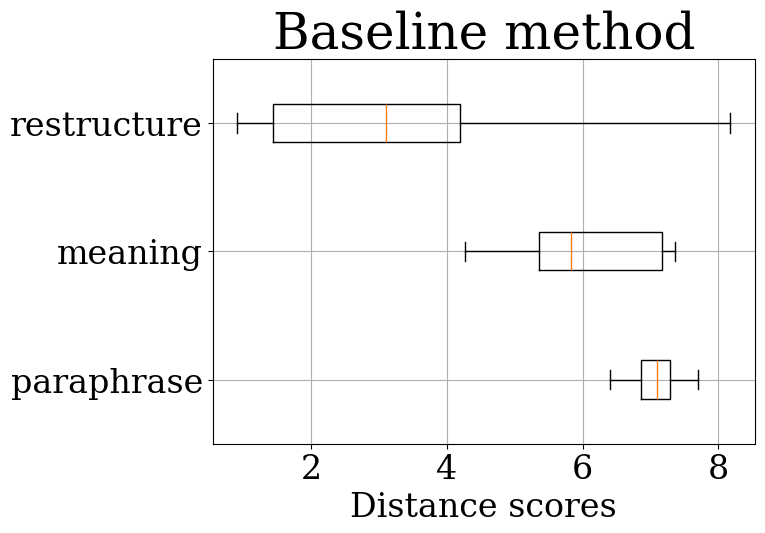
\includegraphics[width=\linewidth]{img/baseline_results.png}
    \caption{Оценки baseline-метода}
    \label{fig:baseline}
\end{subfigure}~
\begin{subfigure}{.5\textwidth}
    \centering
    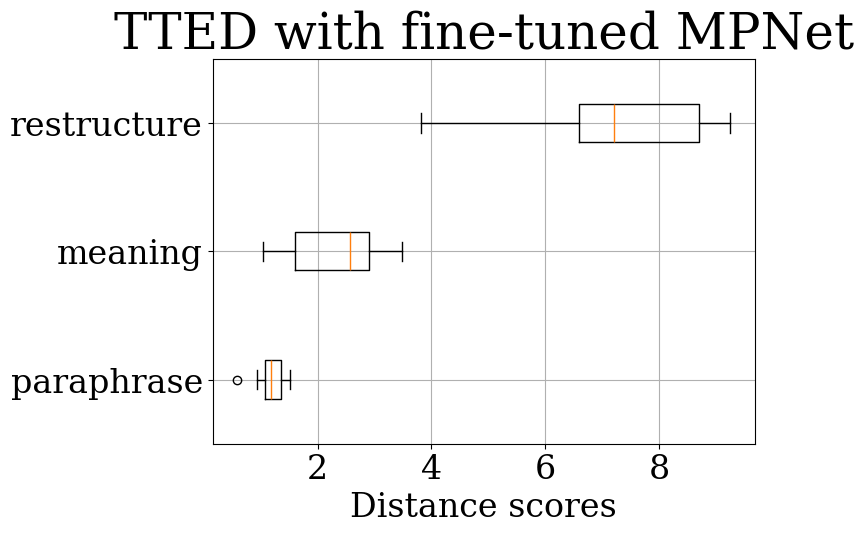
\includegraphics[width=\linewidth]{img/paraphrase_mpnet_results.png}
    \caption{Оценки TTED}
    \label{fig:results}
\end{subfigure}
\caption{Оценки расстояний с помощью TTED и baseline-метода}
\end{figure}

\begin{table}[h]
    \centering
    \begin{tabular}{c|c|c|c|c|c}
        Модель & $\overline{\rho}_1$ & $\overline{\rho}_2$ & $\overline{\rho}_3$ & $R_2(\rho)$ & $R_3(\rho)$ \\ \hline
        Baseline & 7,08$\pm$0,36 & 6,06$\pm$1,04 & 3,61$\pm$2,52 & 1,17$\pm$0,21 & 1,96$\pm$1,37 \\ \hline
        Paraphrase DistilRoBERTa & 2,24$\pm$0,34 & 2,61$\pm$0,60 &	7,52$\pm$1,78 & 0,86$\pm$0,24 & 0,30$\pm$0,08 \\ \hline
        SPECTER & 0,65$\pm$0,16 & 0,83$\pm$0,33 & 2,19$\pm$0,54 & 0,78$\pm$0,37 & 0,30$\pm$0,10 \\ \hline
        MPNet & 1,49$\pm$0,43 & 2,35$\pm$0,87 & 7,09$\pm$1,79 & 0,63$\pm$0,30 & 0,21$\pm$0,08 \\ \hline
        Paraphrase MPNet & 1,18$\pm$0,27 & 2,35$\pm$0,83 & 7,27$\pm$1,65 & \textbf{0,50$\pm$0,21} & \textbf{0,16$\pm$0,05}
    \end{tabular}
    \caption{Средние оценки расстояния с помощью разных языковых моделей}
    \label{tab:model_results}
\end{table}

\begin{table}[h]
    \centering
    \begin{tabular}{c|c|c|c}
        Метод & $\overline{\rho}_1$ & $\overline{\rho}_2$ & $R_2(\rho)$ \\ \hline
        Косинусный коэффициент (без контекста) & 0,14$\pm$0,05 & 0,24$\pm$0,09 & 0,58$\pm$0,31 \\ \hline
        Косинусный коэффициент & 1,18$\pm$0,27 & 2,35$\pm$0,83 & \textbf{0,50$\pm$0,21} \\ \hline
        Евклидово расстояние & 12,92$\pm$1,64 & 17,63$\pm$3,36 & 0,73$\pm$0,17 \\ \hline
        Манхэттенское расстояние & 269,54$\pm$33,37 & 375,88$\pm$71,61 & 0,72$\pm$0,16
    \end{tabular}
    \caption{Средния значения TTED для разных эмбеддинговых расстояний}
    \label{tab:modification_results}
\end{table}

\textit{TO-DO: поставить новый эксперимент по вычислению времени работы}
% Время работы использованных алгоритмов, включая TTED с предподсчетом и без него, представлено в таблице~\ref{tab:compute_time}.

% \begin{table}[h]
%     \centering
% \begin{tabular}{c|c}
%     Метод & Время вычисления, с \\ \hline
%     TTED без предподсчёта & 554,40  \\ \hline
%     TTED с предподсчётом & \textbf{2,18} \\ \hline
%     Baseline & 3,11
% \end{tabular}
%     \caption{Время работы использованных методов на тестовых данных}
%     \label{tab:compute_time}
% \end{table}
        
%%%%%%%%%%%%%%%%%%%%%%%%%%%%%%%%%%%%%%%%%%%%%%%%%%%%%%%%%%%%%%%%%%%%%%%%%%%%%%
\newpage
\section*{Заключение}
\addcontentsline{toc}{section}{\protect\numberline{}Заключение}

\textit{TO-DO}

%%%%%%%%%%%%%%%%%%%%%%%%%%%%%%%%%%%%%%%%%%%%%%%%%%%%%%%%%%%%%%%%%%%%%%%%%
\newpage
\addcontentsline{toc}{section}{\protect\numberline{}Список литературы}
\bibliographystyle{ugost2008}
\bibliography{citations}

\end{document}

